Quests are a massive part of playing the game with tons of content being unlocked by them. Moreover, their large experience rewards drive efficient players to empirically determine the \href{https://oldschool.runescape.wiki/w/Optimal_quest_guide#Quests}{optimal order of completing quests} to obtain any particular goal (most notably the \href{https://oldschool.runescape.wiki/w/Quest_point_cape}{Quest Point Cape}).

The difficulty in optimization arises from the complex dependencies between the quests. To handle this, we can treat each quest as an abstract node. A node has two standard prerequisites: the skill level requirements and the quest requirements. The skill requirements are a property of the node itself, but the quest requirements form edges between these nodes. Since quests reward experience unlocks skill levels, the graph becomes a dynamic, directed acyclic graph (DAG).

Other considerations like item requirements and combat (including bosses) further complicate this process and are not yet considered. Since item requirements can mostly be seen as level requirements, combat becomes the bigger focus. A player could define various constraints for all required combat (eg: $P_\text{win}>0.01$), but this would require modeling equipment progression etc. Although, it would be a major achievement to include all these effects for the purpose of solving the quest problem, for this initial work quests will only depend on skills and other quests.

Quests can only depend on another quest in one direction and as a result they are naturally assigned tiers. For example, tier 0 quests have no quest dependencies, while tier 1 can only depend on Tier 0 quests (or no quests). Each tier depends exclusively on quests in lower tiers. This organizational hierarchy can be seen in Fig.~\ref{fig:quests_by_requirement}.

The \href{https://osrsmath.palfore.com/}{Runescape Universe} is an interactive tool to explore the quest tree in both OSRS and RS3, created by this project to provide users with an interactive way to explore the dynamic, complex, and intertwined quest lines as shown in Fig.~\ref{fig:osrs_universe}. For example, the iconic quest \href{https://oldschool.runescape.wiki/w/Monkey_Madness_I}{Monkey Madness I} is shown in Fig.~\ref{fig:osrs_universe_zoom} to connect to a central network. In fact, all quests are connected to the large central island, except for isolated nodes (typically only 1 or 2 nodes). Only trivial quest islands existed until the \href{https://oldschool.runescape.wiki/w/Varlamore}{Varlamore continent} was released. This island is likely temporary since the same thing happened when the \href{https://oldschool.runescape.wiki/w/Great_Kourend}{Kourend continent} was released, but was later connected to the main island through \href{https://oldschool.runescape.wiki/w/Dragon_Slayer_II}{DSII}.




\begin{figure}
	\centering
	\includegraphics[width=\linewidth]{img/quests/osrs_by_requirement.pdf}
	\caption{
		The OSRS quest tree, which organizes all quests into tiers, with higher tier quests depending exclusively on lower tier quests. With the release of \emph{Song of the Elves} in 2019, OSRS gained a 7th quest tier. By contrast RS3 has 11 tiers (Aftermath and Sliske's Endgame). Edges are colored by the quest tier they unlock. Increasing tiers diminish in size, although this is not required and stems from game design choices.
	}
	\label{fig:quests_by_requirement}
\end{figure}



\begin{figure}
	\centering
	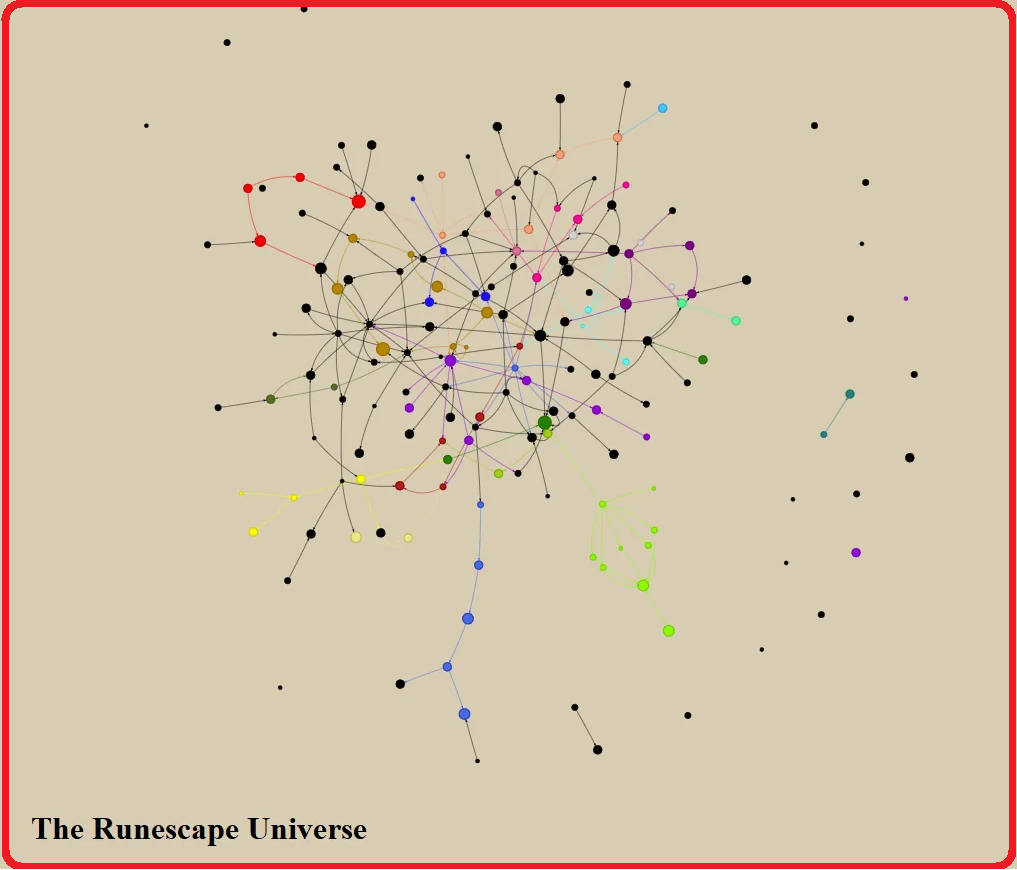
\includegraphics[width=0.8\linewidth]{img/quests/universe.png}
	\caption{
		The Runescape Universe renders all quests and mini-quests as nodes in a graph. The quest prerequisites form edges between the nodes. Isolated islands form quest chains consisting of only one or two nodes. The colors here represent the \href{https://oldschool.runescape.wiki/w/Quests/Series}{quest series} and the size represents the official length of the quest. It is within this picture that nearly all the adventures of our player character are experienced.
	}
	\label{fig:osrs_universe}
\end{figure}




\begin{figure}
	\centering
	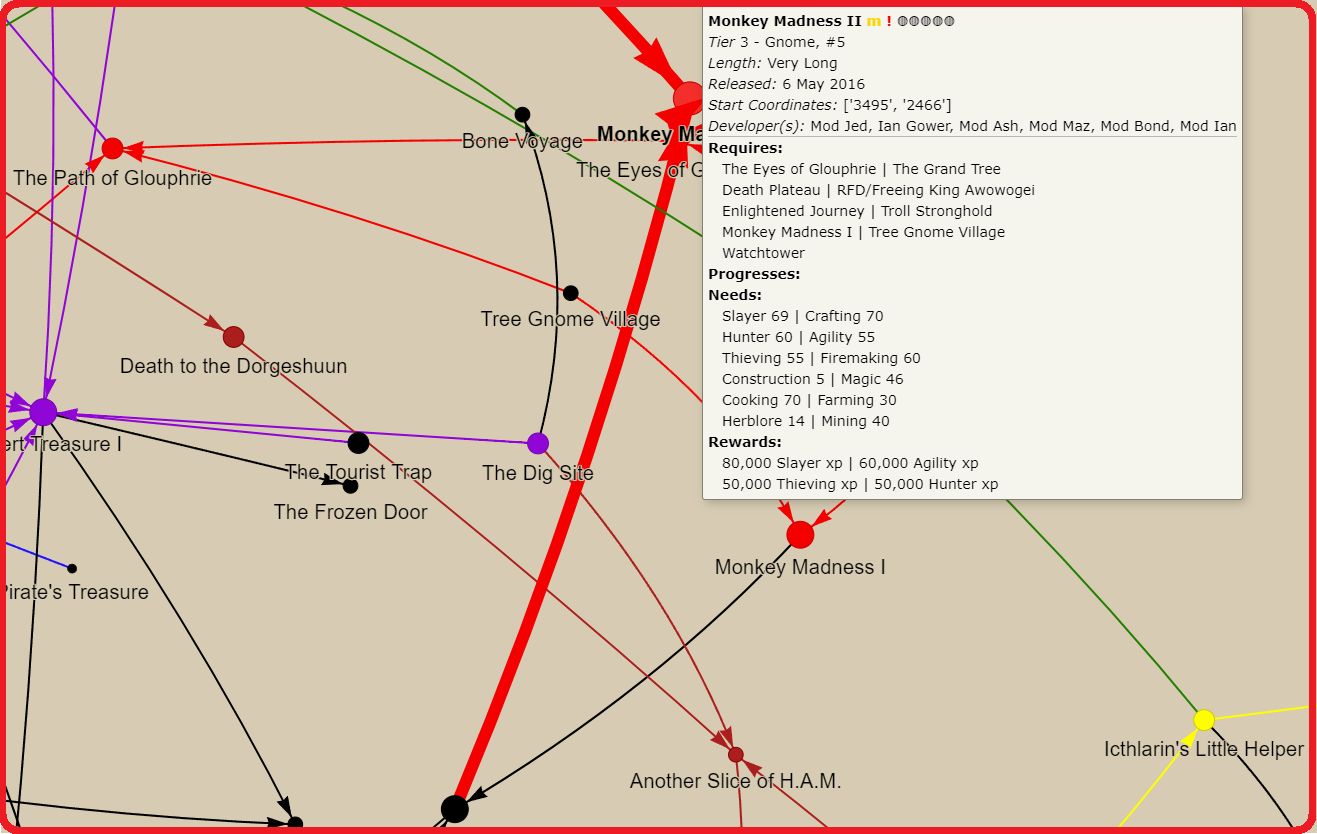
\includegraphics[width=0.8\linewidth]{img/quests/zoom.png}
	\caption{
		A closer view on the Gnome series, which highlights Monkey Madness II, detailing its information in a tooltip. The thick edges represent the direct connections to this quest. Another iconic quest, Desert Treasure I is also pictured. The physical proximity in the graph tends to represent their relatedness i.e. quests in the desert tend to be near each other.
	}
	\label{fig:osrs_universe_zoom}
\end{figure}